% 
% The Topic Browser
% An Interactive Tool for Browsing Topic Models
% Matthew J. Gardner
% Department of Computer Science
% Brigham Young University
% mjg82@byu.edu
% Joshua Lutes
% Department of Computer Science
% Brigham Young University
% jlutes@byu.edu
% Jeff Lund
% Department of Computer Science
% Brigham Young University
% jefflund@gmail.com
% Josh Hansen
% Department of Computer Science
% Brigham Young University
% jjfresh@byu.edu
% Dan Walker
% Department of Computer Science
% Brigham Young University
% danwalkeriv@gmail.com
% Eric Ringger
% Department of Computer Science
% Brigham Young University
% ringger@cs.byu.edu
% Kevin Seppi
% Department of Computer Science
% Brigham Young University
% kseppi@cs.byu.edu
% Abstract
% Topic models have been shown to reveal the semantic content in large corpora.
% Many individualized visualizations of topic models have been reported in the lit-
% erature, showing the potential of topic models to give valuable insight into a cor-
% pus. However, good, general tools for browsing the entire output of a topic model
% along with the analyzed corpus have been lacking. We present an interactive tool
% that incorporates both prior work in displaying topic models as well as some novel
% ideas that greatly enhance the visualization of these models.
% 1
% Introduction
% Proper visualizations are essential to extracting information from and identifying trends in data,
% especially large, high dimensional data. Large text corpora are particularly difficult to visualize, as
% they may include many thousands of documents and millions of words. Topic modeling [1] is a
% method of reducing the dimensionality of a corpus into a set of meaningful topics. Topic models
% have been used with some success as an aid to corpus visualization [3, 9]. However, in many papers
% the presentation of topic models has been limited to hand-selected, coherent topics, when often there
% are many meaningless topics to sift through. These presentations leave the viewer wondering what
% else the topic model discovered and provide little help in gaining a deep understanding of the model.
% To aid in the visualization of topic models and in pattern discovery in document collections, we
% present The Topic Browser, a web-based tool for interactively exploring both the output of a topic
% modeling algorithm and its attendant corpus. Our topic browser incorporates many visualizations of
% topic models previously published as well as some innovative ideas of our own. The Topic Browser
% 
% is an aid both to those who wish to browse through a corpus and for those who wish to analyze
% the topic model itself. We believe that this interactive approach to visualization in browsing reveals
% topics and topical trends in large document collections in a way that is not possible with static
% visualizations. The rest of this paper describes the Topic Browser in an attempt to demonstrate that
% this is true. We display our tool with a topic model run using MALLET’s implementation of LDA [6]
% with 150 topics on a collection of about 460 campaign speeches from the 2008 presidential primary
% and general elections retrieved from http://2008election.procon.org.
% 
% 2
% Extra Information
% Aside from the documents and the topic model themselves, our browser incorporates three other
% pieces of information: attributes (metadata) associated with each document, topic metrics, and doc-
% ument metrics. Here we give a brief description of these kinds of information, deferring a discussion
% of their use in visualization to the subsequent sections.
% Attributes of documents have been used heavily in recent topic models, including the Author-Topic
% model [11], Topics over Time [12], and Dirichlet-Multinomial Regression [7]. While we currently
% do not have specialized visualizations for these topic models, we do include document attributes in
% our browser and have some of our own visualizations that include the attributes.
% In order to browse more effectively through topics, we introduce topic metrics that give information
% about the topic. These range from simple metrics, such as the number of word tokens and types
% labeled with the topic, to more complicated metrics such as how dispersed the topic is across docu-
% ments, or how coherent its words are [10]. We also use pairwise topic metrics as similarity measures
% to show similar topics.
% Similar to topic metrics, one can also compute document metrics. Beyond simple metrics like to-
% ken count in the document, these include things such as the entropy of the topic distribution of
% the document [8]. And as with topics, we make use of pairwise document metrics such as topic
% correlation [3] to show similar documents.
% 
% 3
% Sidebar
% The sidebar in our browser is the main navigation tool. To facilitate navigation through the large
% amount of information in the browser, the sidebar lists the items of the type currently being explored.
% The new capability introduced by this browser is the ability to sort and filter these lists as the user
% desires.
% When presenting the results of a topic model analysis, papers will often hand pick particularly good
% topics to display, leaving out a large number of meaningless topics. While such presentations may
% help to highlight the benefits of a new topic model, they hide the fact that finding good topics is
% often a laborious process. With our topic and document metrics, the sorting and filtering capabilities
% of the sidebar list allow the user to go quickly to meaningful topics that are relevant to his questions.
% When browsing through topics, the user can filter the topic list by coherence to eliminate from
% the view those topics that are mostly meaningless and sort by document entropy (a measure of the
% dispersion of the topic across the documents) to find topics that were used widely throughout the
% corpus. For example, Figure 1 shows that “the family” was one of the most consistent themes in the
% speeches. We use the top two words to name a topic in the sidebar and other places, to avoid clutter,
% though we are actively investigating better ways to name topics.
% The user can also filter by document or attribute to show only topics that were used in a particular
% document or by a particular author. Documents can similarly be filtered and sorted, showing only
% documents that contain tokens with a particular topic or with a particular value of an attribute.
% 4
% Topic Browsing
% The results from a topic model are typically presented as static lists of words, often simply showing
% the top ten words from each topic in a list [1]. While this practice is often sufficient to give a reader
% 
% Figure 1: The navigational sidebar showing topics. In this example the topics are sorted by disper-
% sion throughout the corpus and filtered by coherence
% 
% a basic idea of what the topic captured, it is largely incapable of conveying a deep understanding of
% the context of that topic in the corpus. In order to answer significant questions about a corpus one
% must browse the topics discovered, and previous methods have failed to adequately allow the user
% to explore topics. Our browser presents new ways to gather information about a topic in the corpus,
% both in terms of how the words in the topic are displayed and in terms of what is presented about the
% topic.
% 
% 4.1 Showing Top Words
% Instead of showing a list of the top ten words, we show a word cloud of the top 100, where the
% size of each word is determined by the probability of seeing that word in the topic. We also show a
% re-weighted word cloud as determined by Blei & Lafferty’s Turbo Topics method [4].
% While these visualizations are modest improvements over typical visualization methods, our most
% useful display of the words is showing them in their context. The topics in a topic model cannot
% be fully interpreted when completely separated from their context. Thus in addition to the word
% cloud we also display the top ten words in the topic inside of their context. We select a random
% token of each word type labeled with the topic and show up to 50 characters on either side of the
% token, keeping words intact. We also allow the user to cycle through contexts to gain a broader view
% of how each word is actually used in that topic. When viewing the topic about troops in Iraq, for
% example (see Figure 2), one can see that most often when the word “troops” is used in this topic, it
% is in reference to bringing the troops home, and when “end” is used, it is not used in the context of
% “end the war” as often as one might expect.
% 
% 4.2 Getting More Information
% The browser provides two main ways of getting more information about topics in the model. The
% first is showing documents and attribute values which have either the highest number of tokens
% labeled with that topic or the highest proportion (by percentage) of the given topic. This allows
% 
% Figure 2: The top ten words in the topic shown with a random context selected from the corpus.
% Figure 3: Part of the overall topic view, looking at a topic about education. Note particularly the top
% documents for the topic and the top values for the attribute “party,” shown at the bottom.
% 
% the user to quickly find documents that best demonstrate what the topic captured. Showing the top
% values for a given attribute (such as authors for the attribute “Author”) gives the user an idea of how
% focused the topic is and often reveals interesting information about the corpus being browsed. For
% example, in Figure 3, we see that Democrats spoke more often about education than Republicans
% did, at least in the topic shown.
% The other way that we give more information about topics is by showing similar topics. We find sim-
% ilar topics either by looking at the distribution of documents that contain the topic or by the topic’s
% distribution over words. Looking at similar topics by document shows topics that are commonly
% used together in the corpus, and finding similar topics by word distribution shows topics that have
% similar words, possibly because the two topics really should have been one topic. When looking at
% a topic about health care, the user can see that other topics used together with the health care topic
% include topics about the cost of medication and the quality of care (see Figure 4).
% 
% 5
% Document, Word, and Attribute Browsing
% In addition to enabling the user to browse the topics in the topic model, we provide means for
% browsing the documents, words, and attributes in the corpus. These facilities give users the ability
% to explore the corpus itself in the context of the topic model.
% 
% Figure 4: Another look at the overall topic view, featuring different parts of the view. Note particu-
% larly the similar topics box near the top right.
% 
% When simply browsing through the documents, we provide sorting and filtering methods on the list
% of documents, as mentioned previously. When looking at a particular document, we show basic in-
% formation about the document, its text, the topic distribution in the document, and similar documents
% based on that distribution. When looking at the document in the context of a topic, we also highlight
% the tokens in the document that were labeled with that topic. For example, the user might be curious
% to see a document that best demonstrates the health care topic mentioned above. Clicking on the top
% document in the document list (as in the bottom of Figure 3) brings the user to the view shown in
% Figure 5.
% The document visualizations reported here were drawn from the work of others [1], and in fact the
% view in Figure 5 constitutes the entirety of most previous corpus browsers based on topic models
% (e.g., [2]). Our browser substantially goes beyond the existing functionality reported by others.
% We also provide views of individual words in the corpus. When viewing a word in the context of a
% topic, the user can see all uses of the word in that topic in the corpus, with context taken from their
% corresponding documents. The user can also view words independently with a search-like interface,
% seeing topics and documents in which the word appears most frequently. The user examining the
% health care topic might be curious where else the word “health” was used in the topics and in the
% corpus. Figure 6 shows the result of using our word search to answer that question. While providing
% basic functionality, however, the search interface leaves much to be desired, as only single words
% can currently be searched for. We plan on expanding that to phrases.
% The user can also look at aggregated information for the values of an attribute (i.e., a particular
% candidate or party), combining all of the topic and word counts for all documents with the given
% attribute. This view is also at present somewhat limited, showing only what topics and words are
% used most frequently by the collection of documents with that attribute. Figure 7 shows us, among
% other things, that one of Barack Obama’s top topics was “change in politics.”
% 
% 6
% Plots
% We currently include two kinds of plots in our topic browser, with plans to implement many more.
% The first shows trends for topics over the values of an attribute (such as date, or candidate), useful
% for corpus browsing. This kind of plot has been used in visualizing topic models almost since their
% 
% Figure 5: The document view, looking at a speech by Hillary Clinton in the context of a topic about
% health care (the rest of the document is cut off in this screenshot, and sadly, the colored tokens in the
% document are not very visible in black and white).
% Figure 6: The word search functionality, showing the results for searching for the word “health.”
% 
% Figure 7: The attribute view, showing aggregated information for all speeches given by Barack
% Obama.
% Figure 8: A plot of topics over attributes, showing the use of three health care-related topics across
% candidates.
% introduction [5]. Our topic browser allows the user to interactively generate these trend plots over
% any attribute for any topic or combination of topics in the corpus. Our user exploring health care
% topics may want to view how much each candidate spoke about health care. We saw already that
% there were three related topics that mentioned health care, so the user might view all of them together
% in a histogram, shown in Figure 8.
% The second kind of plot that we include is more useful for analyzing and understanding the behavior
% of the topic model itself. We allow the user to plot two topic metrics against each other and compute
% a linear regression. This allows the user to see some interesting properties of the topic metrics, such
% as the fact that document entropy seems to correlate with the logarithm of the number of tokens in
% the topic, and that coherence does not seem to correlate with any other topic metric. The user can
% also find outliers, such as topics with low document entropy but a high token count, that can then be
% examined in the topic page.
% An interesting application of these topic metric plots occurs when the metrics include how con-
% sistently each candidate spoke about each topic. Figure 9 shows a plot of topics, comparing John
% McCain’s use of each topic to Barack Obama’s use of the topic. Topics in the upper left were topics
% unique to Obama, and topics in the lower right were unique to McCain. Topics in the middle (near
% the value of 2 for each candidate) were somewhat shared between the two.
% 7
% Figure 9: A topic metric comparison plot. The metrics plotted are how consistently Barack Obama
% and John McCain used each topic. The plot shows topics that were unique to Obama or McCain and
% topics they shared.
% 7
% Conclusion
% We have presented the Topic Browser, an interactive tool for browsing both the output of a topic
% model and the corpus that was modeled. We have shown that our tool incorporates many previously
% published visualizations of topic models, including basic corpus browsing functionality, plots of
% trends over attributes in the corpus, the use of coherence to ignore meaningless topics, and Blei &
% Lafferty’s Turbo Topics method of finding significant phrases for each topic. We have also presented
% many novel ways to mine information from a topical analysis of a corpus in an interactive browsing
% experience. The Topic Browser is an effective tool both for those wishing to browse through a corpus
% in the context of a topic model, and for those wishing to better understand topic models and develop
% new models.
% While our tool is still under development, a description of the Topic Browser, a working demo,
% and the current version of the code are available at http://nlp.cs.byu.edu/topic browser. Our tool
% currently supports any topic model that labels individual tokens in the corpus with topics, and is
% built to import data directly from MALLET input and output files [6], or files similarly formatted.
% We have plans to include specialized visualizations for more complicated topic models, such as
% Topics over Time, sentiment-topic models, hierarchical topic models, and others.
% References
% [1] David M. Blei, Andrew Y. Ng, and Michael I Jordan. Latent dirichlet allocation. Journal of
% Machine Learning Research, 3:993–1022, 2003.
% [2] D.M. Blei.
% 50-topic-browser of latent Dirichlet allocation fit to the 2006 arXiv.
% http://topics.cs.princeton.edu/arxiv/browser50/. Accessed 10/21/2010.
% [3] D.M. Blei and J.D. Lafferty. Topic Models. In Ashok Srivastava and Mehran Sahami, editors,
% Text Mining: Classification, Clustering, and Applications. Taylor and Francis, 2009.
% [4] D.M. Blei and J.D. Lafferty.
% Visualizing Topics with Multi-Word Expressions.
% arXiv:0907.1013v1 [stat.ML], 2009.
% [5] T.L. Griffiths and M. Steyvers. Finding scientific topics. Proceedings of the National Academy
% of Sciences, 101(Suppl 1):5228, 2004.
% [6] Andrew Kachites McCallum. MALLET: A Machine Learning for Language Toolkit, 2002.
% [7] D. Mimno and A. McCallum. Topic models conditioned on arbitrary features with dirichlet-
% multinomial regression. In Proceedings of the 24th Annual Conference on Uncertainty in
% Artificial Intelligence. Citeseer, 2008.
% [8] H. Misra, O. Capp´ , and F. Yvon. Using LDA to detect semantically incoherent documents. In
% e
% Proceedings of the Twelfth Conference on Computational Natural Language Learning, pages
% 41–48. Association for Computational Linguistics, 2008.
% 8
% [9] D. Newman, T. Baldwin, L. Cavedon, E. Huang, S. Karimi, D. Martinez, F. Scholer, and J. Zo-
% bel. Visualizing search results and document collections using topic maps. Web Semantics:
% Science, Services and Agents on the World Wide Web, 2010.
% [10] D. Newman, J.H. Lau, K. Grieser, and T. Baldwin. Automatic evaluation of topic coherence.
% In NAACL HLT, 2010.
% [11] M. Rosen-Zvi, T. Griffiths, M. Steyvers, and P. Smyth. The author-topic model for authors
% and documents. In Proceedings of the 20th conference on Uncertainty in artificial intelligence,
% page 494. AUAI Press, 2004.
% [12] X. Wang and A. McCallum. Topics over time: a non-Markov continuous-time model of topical
% trends. In Proceedings of the 12th ACM SIGKDD international conference on Knowledge
% discovery and data mining, pages 424–433. ACM, 2006.
% 9


% \documentclass[a4paper,10pt]{article}
% \usepackage[utf8x]{inputenc}
% 
% 
% %opening
% \title{Exploring Your Favorite Corpus with The Topic Browser}
% \author{}
% 
% \begin{document}
% 
% \maketitle
% 

% % 
% % \section{Why?}

% % 
% % Previous visualization attempts....
% % 
% % Why they fail
% % 
% % 
% % 
% % 
% % 
% % \subsection{...but their output is hard for humans to digest}
% % \subsection{Topics aren't isolated entities, but form a network in combination
% % with documents, words, authors, etc.}
% % \subsection{This network is implied by a topic model, but generally not made
% % explicit (?)}
% % \subsection{More informative}
% % Experience suggests that an explicit representation of the relationships between
% % all entities modeled and makes topic model output more informative and usable.
% % [We're in the process of formally validating this claim.]
% % 

% 
% 
% 
% 
% 
% \end{document}

%
% File acl-hlt2011.tex
%
% Contact: gdzhou@suda.edu.cn
%%
%% Based on the style files for ACL2008 by Joakim Nivre and Noah Smith
%% and that of ACL2010 by Jing-Shin Chang and Philipp Koehn


\documentclass[11pt]{article}
\usepackage{acl-hlt2011}
\usepackage{times}
\usepackage{latexsym}
\usepackage{amsmath}
\usepackage{multirow}
\usepackage{url}
\usepackage{graphicx}
\DeclareMathOperator*{\argmax}{arg\,max}
\setlength\titlebox{6.5cm}    % Expanding the titlebox

\title{Exploring Your Favorite Corpus with The Topic Browser}
\author{Matthew J. Gardner, Joshua Lutes, Josh Hansen, Jeff Lund, Dan Walker, Eric Ringger, \and Kevin Seppi\\
Department of Computer Science\\
Brigham Young University\\
\tt \{mjg82,jlutes,joshhansen\}@byu.edu, \{jefflund,danwalkeriv\}@gmail.com\\
\tt \{ringger,kseppi\}@cs.byu.edu}

\date{}

\begin{document}
\maketitle

% \begin{abstract}
% Problem: You're developing yet another LDA variant and want to get a feel for its output.
% Solution: Use the Topic Browser to check things out at the topic, word, and document levels.
% Problem: You have a mountain of documents so vast that no non-cyborg could read them all.
% Solution: Get the Topic Browser and do some interactive, topic-based exploration.
% Problem: The public has difficulty accessing the treasure trove of documents your institution wishes to make available.
% Solution: Expose it to the world via the Topic Browser's web interface.
% \end{abstract}

\begin{abstract}
The Topic Browser is an open-source\footnote{Licensed under the terms of the
Affero General Public License, version 3.}  web application for interactive
exploration and visualization of topics and documents. Mallet LDA output is used
as input. We explain why such a tool is warranted, what it is capable of, and
how to use it to explore the corpus (or topic model) of your choice.
\end{abstract}

\section{Introduction}
Since their introduction in 2003, LDA-based topic models have been extended to
account for time, authors, citations, multiple languages, etc. [][][][][]
Baseline LDA generates a topic assignment per (non-stop) token -- a massive
output in the gigaword era. Humans are incapable of fully assimilating the
resulting models, calling for more effective means of characterizing and
visualizing the output.

The Topic Browser is an open-source web application for interactive exploration
and visualization of document collections. All entities implied by topic model output are first-class citizens in the Topic
Browser. 

% \subsection{Entities}
% \begin{figure}[ht]
%  \centering
%  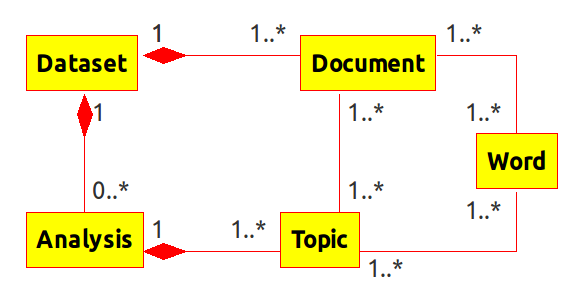
\includegraphics{topic_browser_object_model_transparent.png}
%  % topic browser object model transparent.png: 582x293 pixel, 96dpi, 15.40x7.75
% cm, bb=0 0 436 220
%  \caption{The Topic Browser object model}
%  \label{fig:object_model}
% \end{figure}

\subsection{Topics}

\subsection{Documents}

\subsection{Words}

\subsection{Metrics}
Topic-centric document exploration is enhanced by means of \textit{metrics}.\footnote{These do not necessarily constitute ``metrics'' in the formal sense.} Metrics describe either topics or documents and come in two flavors: unary and binary (or pairwise). 

% topic, topic-topic, document, document-document
% if 'topic_metrics' not in locals():
%     topic_metrics = ["token count", "type count", "document entropy", "word entropy"]
% if 'pairwise_topic_metrics' not in locals():
%     pairwise_topic_metrics = ["document correlation", "word correlation"]
% if 'document_metrics' not in locals():
%     document_metrics = ['token count', 'type count', 'topic entropy']
% if 'pairwise_document_metrics' not in locals():
%     pairwise_document_metrics = ['word correlation','topic correlation']
% if 'name_schemes' not in locals():
%     name_schemes = [
%                TopNTopicNamer(dataset_name, analysis_name, 2),
% #               TfitfTopicNamer(dataset_name, analysis_name, 5)
%                ]
\subsection{Charts}



\subsection{Topic ``Maps"}
With topic-to-topic relationships described by means of pairwise topic metrics,
graph-based visualization of the topic space becomes straightforward. In our
current implementation, we construct a topic graph G = (N, E) as follows:
\begin{itemize}
\item $N$ is a set of $|T|$ nodes such that $\forall_{t\in T} weight(N_{t}) =
\tau(t)$ where $\tau$ is a topic metric.
\item $E$ is a set of $|T|^2$ edges such that $\forall_{t\in T}\forall_{u\in T}
weight(E_{t,u}) = \mu(t,u)$ where $\mu$ is a pairwise topic metric.
\end{itemize}

We use the Gephi Toolkit\footnote{http://www.gephi.org} to generate such graphs
and render them as images.
% \begin{figure}
%   \begin{center}
%   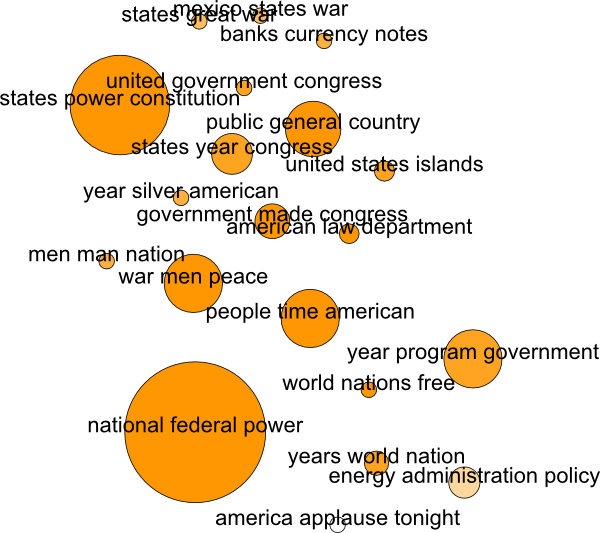
\includegraphics[width=200px,keepaspectratio=true]{./topic_map_example.png}
%   \caption{}
%   \end{center}
% \end{figure}
% \begin{center}
%  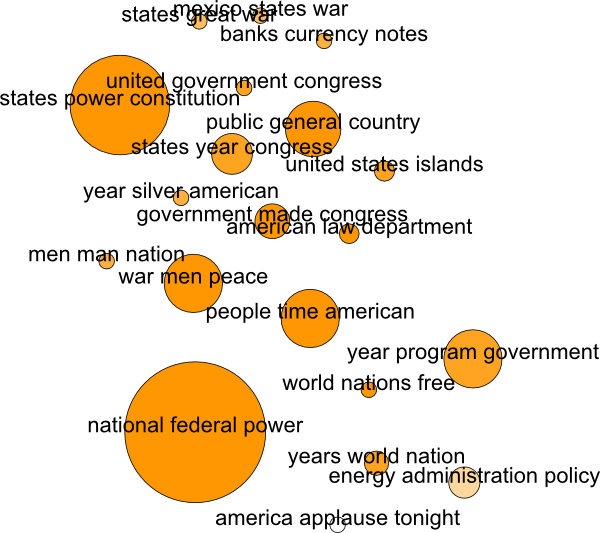
\includegraphics[width=200px,keepaspectratio=true]{./topic_map_example.png}
%  % topic_map_example.png: 600x533 pixel, 57dpi, 26.76x23.77 cm, bb=0 0 759 674
% \end{center}

\begin{figure}[p]
 \centering
 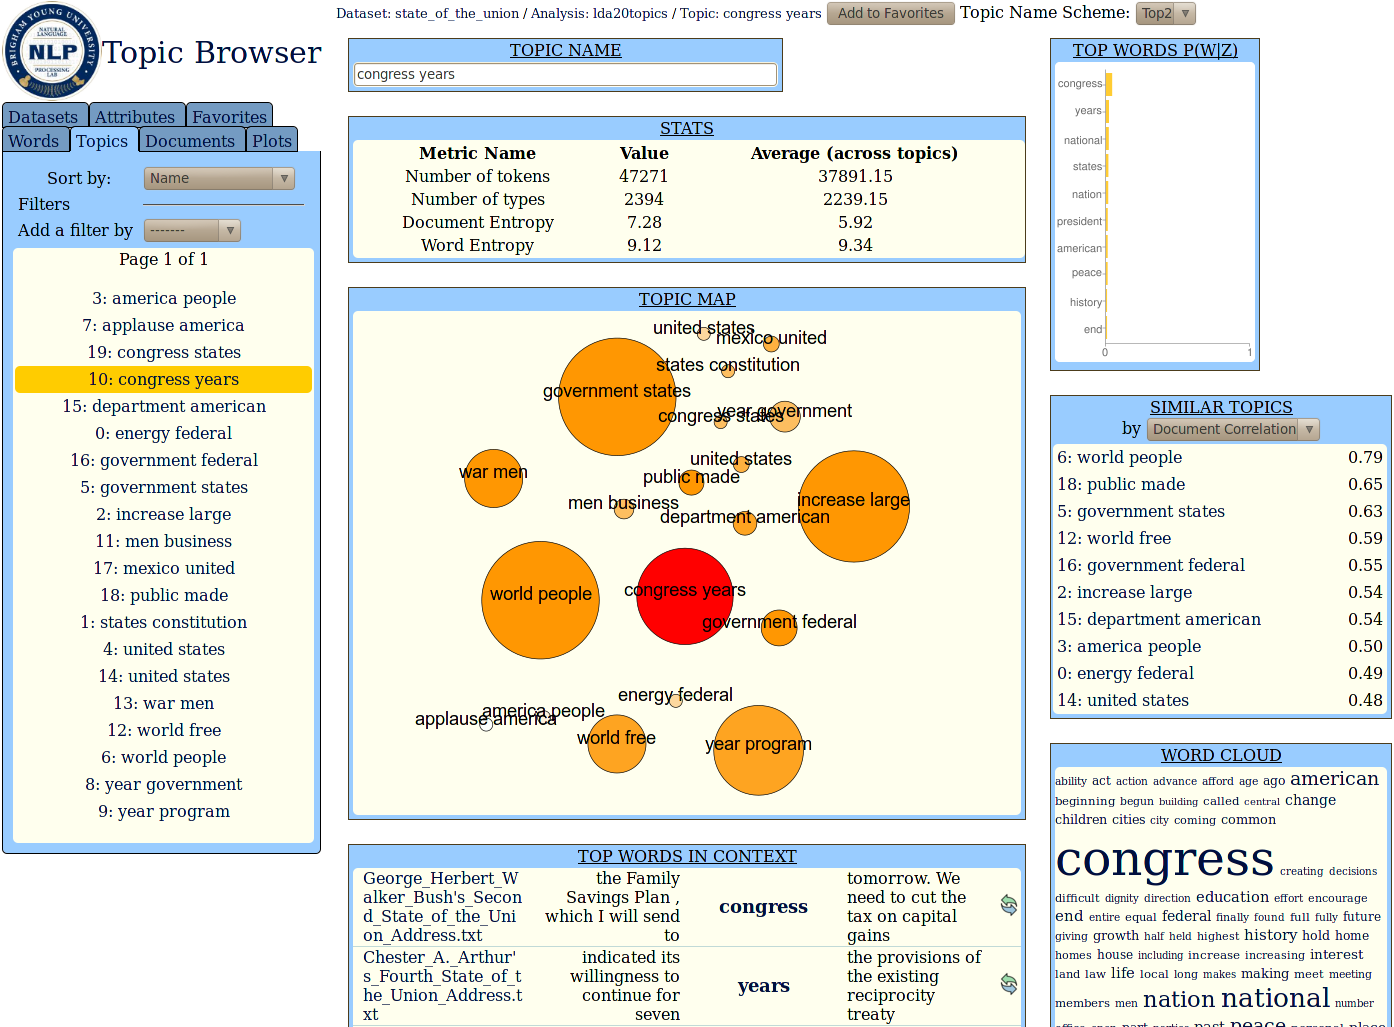
\includegraphics[width=400px,keepaspectratio=true]{./topic_page_huge_cropped.png}
 % topic_page_huge_cropped.png: 1394x1027 pixel, 96dpi, 36.88x27.17 cm, bb=0 0 1045 770
 \caption{The topic page}
 \label{fig:topic_page}
\end{figure}

\subsection{Topic Name Schemes}
As LDA does not assign names to the topics it generates, automatic generation of
topic names is of interest to researchers wishing to make topic models
human-usable. Research in this area is ongoing (CITATION???). In order to
facilitate investigations in this area, we equipped the Topic Browser with a
fully pluggable topic naming system. Any number of topic name schemes can be
used to produce names for all topics in an analysis. Within the user interface
users can select a name scheme, which is then reflected throughout the
interface. By default we use ''Top2`` (the name is a concatenation of the two
words with the highest $P(w|z)$ for a given topic $z$), but any number of
alternative schemes can be imagined and implemented. (MAYBE SHOW TF-ITF?)

\section{Data Import Backend}
SHOW DEPENDENCY GRAPH?
Automatically turning a raw document collection into an interactive browsing
experience requires extensive preprocessing. Documents must be converted into a
representation accepted by the topic model learner. Topics must then be inferred
and model output indexed. Additionally, metrics must be computed, topic names
generated, and graphs rendered before they become accessible via the user
interface. Unsurprisingly, the dependencies in the import process form a DAG. To
improve the efficiency and usability of the data import pipeline we built a
command-line frontend based on the \verb/doit/ task automation tool, written in
Python.\footnote{http://doit.sourceforge.net/}

The main \verb/doit/ build script is \verb/dodo.py/. Some example invocations:
\begin{itemize}
 \item \verb/dodo.py/: Builds all targets
 \item \verb/dodo.py list/: Lists the available top-level tasks (sub-tasks are not displayed)
 \item \verb/dodo.py clean -c mallet/: Cleans the Mallet files
\end{itemize}

% Useful commands:
%  dodo.py list #Lists the available top-level tasks (sub-tasks are not displayed)
%  dodo.py #Builds everything!
%  dodo.py clean -c mallet #Cleans the mallet files
%  dodo.py metrics #Computes all metrics
%  dodo.py topic_metrics #Computes just the topic metrics
%  dodo.py topic_metrics:document_entropy #Computes just the document entropy topic metric
%  dodo.py clean topic_metrics:document_entropy #Cleans just the document entropy topic metric
%
%NOTE: probably necessary to do 'dodo.py forget' when switching between datasets/analyses.

how to set different datasets

\subsection{Adding Support For Your Dataset}
The \verb/build/ Python module contains dataset-specific import scripts.
Generally, a sub-module contains the scripts for a particular dataset. The
scripts for the default State of the Union Addresses dataset, for example,
reside in \verb/build.state_of_the_union/. The main build file for the dataset
is \verb#build/state_of_the_union/state_of_the_union.py#. This file is
referenced within the root \verb/dodo.py/ build script by setting the
\verb/build/ variable:
\begin{verbatim}
 build = "state_of_the_union/state_of_the_union"
\end{verbatim}

At a minimum, the dataset-specific build file should contain the following:
\begin{itemize}
 \item Declaration of \verb/dataset_name/ variable.
   \newline Example: \verb/dataset_name = "state_of_the_union"/.
 \item Declaration of \verb/dataset_description/ variable.
   \newline Example: \verb/dataset_description = "State of the Union Addresses 1790-2010"/.
 \item Definition of \verb/copy_and_transform_dataset/ \verb/doit/ task.
Example:
\begin{verbatim}
def task_copy_and_transform_dataset():
  task = dict()
  task['actions'] = [
    (extract_state_of_the_union,
    [dataset_dir+'/'+chron_list_filename,
     dataset_dir+'/'+addresses_filename,
     files_dir]
    )
  ]
  task['clean'] = [
    'rm -rf '+files_dir
  ]
  task['uptodate'] = [os.path.exists(files_dir)]
  return task
\end{verbatim}

\end{itemize}

% \section{Credits}
% 
% This document has been adapted from the instructions for earlier ACL proceedings, including those for ACL-2008 by Johanna D. Moore, Simone Teufel, James Allan, and Sadaoki Furui, those for ACL-2005 by Hwee Tou Ng and Kemal Oflazer, those for ACL-2002 by Eugene Charniak and Dekang Lin, and earlier ACL and EACL formats. Those versions were written by several people, including John Chen, Henry S. Thompson and Donald Walker. Additional elements were taken from the formatting instructions of the {\em International Joint Conference on Artificial Intelligence}.
% 
% \section{Introduction}
% 
% The following instructions are directed to authors of papers submitted to ACL-HLT-2011 or accepted for publication in its proceedings. All authors are required to adhere to these specifications. Authors are required to provide a Portable Document Format (PDF)
% % das: removed reference to PostScript
% % and PostScript
% version of their papers. \textbf{The proceedings will be printed on US-Letter paper}. Authors from countries in which access to word-processing systems is limited should contact the publication chair Guodong Zhou ({\tt gdzhou@suda.edu.cn}) as soon as possible.
% 
% 
% \section{General Instructions}
% 
% Manuscripts must be in two-column format. Exceptions to the two-column format include the title, authors' names and complete addresses, which must be centered at the top of the first page, and any full-width figures or tables (see the guidelines in Subsection~\ref{ssec:first}). {\bf Type single-spaced}. Start all pages directly under the top margin. See the guide-lines later regarding formatting the first page.
% 
% The maximum length of a manuscript is eight (8) pages for the main conference, printed single-sided, plus two (2) pages for references (see Section~\ref{sec:length} for additional information on the maximum number of pages).  Do not number the pages.
% 
% \subsection{Electronically-available resources}
% 
% ACL-HLT-2011 provides this description in \LaTeX2e (acl-hlt2011.tex) and PDF format (acl-hlt2011.pdf), along with the LATEX2e style file used to format it (acl-hlt2011.sty) and an ACL bibliography style (acl.bst). These files are all available at \url{http://www.acl2011.org}.  A Microsoft Word template file (acl-hlt2011.dot) is also available at the same URL. We strongly recommend the use of these style files, which have been appropriately tailored for the ACL-HLT-2011 proceedings. If you have an option, we recommend that you use the \LaTeX2e version. \textbf{If you will be using the Microsoft Word template, we suggest that you anonymize your source file so that the pdf produced does not retain your identity.} This can be done by removing any personal information from your source
% document properties.
% 
% 
% \subsection{Format of Electronic Manuscript}
% \label{sect:pdf}
% 
% For the production of the electronic manuscript you must use Adobe's
% Portable Document Format (PDF). This format can be generated from
% postscript files: on Linux/Unix systems, you can use {\tt ps2pdf} for this
% purpose; under Microsoft Windows, you can use Adobe's Distiller, or
% if you have {\tt cygwin} installed, you can use {\tt dvipdf} or
% {\tt ps2pdf}.  Note
% that some word processing programs generate PDF which may not include
% all the necessary fonts (esp. tree diagrams, symbols). When you print
% or create the PDF file, there is usually an option in your printer
% setup to include none, all or just non-standard fonts.  Please make
% sure that you select the option of including ALL the fonts.  {\em Before sending it, test your PDF by printing it from a computer different from the one where it was created}. Moreover,
% some word processor may generate very large postscript/PDF files,
% where each page is rendered as an image. Such images may reproduce
% poorly.  In this case, try alternative ways to obtain the postscript
% and/or PDF.  One way on some systems is to install a driver for a
% postscript printer, send your document to the printer specifying
% ``Output to a file'', then convert the file to PDF.
% 
% Additionally, it is of utmost importance to specify the {\bf US-Letter format} (8.5in $\times$ 11in) when formatting the paper. When working with {\tt dvips}, for instance, one should specify {\tt -t letter}.
% 
% Print-outs of the PDF file on US-Letter paper should be identical to the
% hardcopy version.  If you cannot meet the above requirements about the
% production of your electronic submission, please contact the
% publication chair above as soon as possible.
% 
% 
% \subsection{Layout}
% \label{ssec:layout}
% 
% Format manuscripts two columns to a page, in the manner these
% instructions are formatted. The exact dimensions for a page on US-letter
% paper are:
% 
% \begin{itemize}
% \item Left and right margins: 1in
% \item Top margin:1in
% \item Bottom margin: 1in
% \item Column width: 3.15in
% \item Column height: 9in
% \item Gap between columns: 0.2in
% \end{itemize}
% 
% \noindent Papers should not be submitted on any other paper size. If you cannot meet the above requirements about the production of your electronic submission, please contact the publication chair above as soon as possible.
% 
% \subsection{Fonts}
% 
% For reasons of uniformity, Adobe's {\bf Times Roman} font should be
% used. In \LaTeX2e{} this is accomplished by putting
% 
% \begin{quote}
% \begin{verbatim}
% \usepackage{times}
% \usepackage{latexsym}
% \end{verbatim}
% \end{quote}
% in the preamble. If Times Roman is unavailable, use {\bf Computer
%   Modern Roman} (\LaTeX2e{}'s default).  Note that the latter is about
%   10\% less dense than Adobe's Times Roman font.
% 
% 
% \begin{table}[h]
% \begin{center}
% \begin{tabular}{|l|rl|}
% \hline \bf Type of Text & \bf Font Size & \bf Style \\ \hline
% paper title & 15 pt & bold \\
% author names & 12 pt & bold \\
% author affiliation & 12 pt & \\
% the word ``Abstract'' & 12 pt & bold \\
% section titles & 12 pt & bold \\
% document text & 11 pt  &\\
% captions & 11 pt & \\
% abstract text & 10 pt & \\
% bibliography & 10 pt & \\
% footnotes & 9 pt & \\
% \hline
% \end{tabular}
% \end{center}
% \caption{\label{font-table} Font guide. }
% \end{table}
% 
% \subsection{The First Page}
% \label{ssec:first}
% 
% Center the title, author's name(s) and affiliation(s) across both
% columns. Do not use footnotes for affiliations.  Do not include the
% paper ID number assigned during the submission process.
% Use the two-column format only when you begin the abstract.
% 
% {\bf Title}: Place the title centered at the top of the first page, in
% a 15 point bold font.  (For a complete guide to font sizes and styles, see Table~\ref{font-table}.)
% Long title should be typed on two lines without
% a blank line intervening. Approximately, put the title at 1in from the
% top of the page, followed by a blank line, then the author's names(s),
% and the affiliation on the following line.  Do not use only initials
% for given names (middle initials are allowed). Do not format surnames
% in all capitals (e.g., ``Zhou,'' not ``ZHOU'').  The affiliation should
% contain the author's complete address, and if possible an electronic
% mail address. Leave about 0.75in between the affiliation and the body
% of the first page. The title, author names and addresses should be completely identical to those entered to the electronic paper submission website in order to maintain the consistency of author information among all publications of the conference.
% 
% {\bf Abstract}: Type the abstract at the beginning of the first
% column.  The width of the abstract text should be smaller than the
% width of the columns for the text in the body of the paper by about
% 0.25in on each side.  Center the word {\bf Abstract} in a 12 point
% bold font above the body of the abstract. The abstract should be a
% concise summary of the general thesis and conclusions of the paper.
% It should be no longer than 200 words. The abstract text should be in 10 point font.
% 
% {\bf Text}: Begin typing the main body of the text immediately after
% the abstract, observing the two-column format as shown in
% the present document. Do not include page numbers.
% 
% {\bf Indent} when starting a new paragraph. For reasons of uniformity,
% use Adobe's {\bf Times Roman} fonts, with 11 points for text and
% subsection headings, 12 points for section headings and 15 points for
% the title.  If Times Roman is unavailable, use {\bf Computer Modern
%   Roman} (\LaTeX2e's default; see section \ref{sect:pdf} above).
% Note that the latter is about 10\% less dense than Adobe's Times Roman
% font.
% 
% \subsection{Sections}
% 
% {\bf Headings}: Type and label section and subsection headings in the
% style shown on the present document.  Use numbered sections (Arabic
% numerals) in order to facilitate cross references. Number subsections
% with the section number and the subsection number separated by a dot,
% in Arabic numerals. Do not number subsubsections.
% 
% {\bf Citations}: Citations within the text appear
% in parentheses as~\cite{Gusfield:97} or, if the author's name appears in
% the text itself, as Gusfield~\shortcite{Gusfield:97}. Append lowercase letters to the year in cases of ambiguities. Treat double authors as in~\cite{Aho:72}, but write as in~\cite{Chandra:81} when more than two authors are involved. Collapse multiple citations as in~\cite{Gusfield:97,Aho:72}. Also refrain from using full citations as sentence constituents. We suggest that instead of
% \begin{quote}
%   ``\cite{Gusfield:97} showed that ...''
% \end{quote}
% you use
% \begin{quote}
% ``Gusfield \shortcite{Gusfield:97}   showed that ...''
% \end{quote}
% 
% If you are using the provided \LaTeX{} and Bib\TeX{} style files, you
% can use the command \verb|\newcite| to get ``author (year)'' citations.
% 
% As reviewing will be double-blind, the submitted version of the papers should not include the
% authors' names and affiliations. Furthermore, self-references that
% reveal the author's identity, e.g.,
% \begin{quote}
% ``We previously showed \cite{Gusfield:97} ...''
% \end{quote}
% should be avoided. Instead, use citations such as
% \begin{quote}
% ``Gusfield \shortcite{Gusfield:97}
% previously showed ... ''
% \end{quote}
% 
% Please do not  use anonymous
% citations and  do not include acknowledgements when submitting your papers. Papers that do not conform
% to these requirements may be rejected without review.
% 
% \textbf{References}: Gather the full set of references together under
% the heading {\bf References}; place the section before any Appendices,
% unless they contain references. Arrange the references alphabetically
% by first author, rather than by order of occurrence in the text.
% Provide as complete a citation as possible, using a consistent format,
% such as the one for {\em Computational Linguistics\/} or the one in the
% {\em Publication Manual of the American
% Psychological Association\/}~\cite{APA:83}.  Use of full names for
% authors rather than initials is preferred.  A list of abbreviations
% for common computer science journals can be found in the ACM
% {\em Computing Reviews\/}~\cite{ACM:83}.
% 
% The \LaTeX{} and Bib\TeX{} style files provided roughly fit the
% American Psychological Association format, allowing regular citations,
% short citations and multiple citations as described above.
% 
% {\bf Appendices}: Appendices, if any, directly follow the text and the
% references (but see above).  Letter them in sequence and provide an
% informative title: {\bf Appendix A. Title of Appendix}.
% 
% \textbf{Acknowledgment} sections should go as a last section immediately
% before the references. Do not number the acknowledgement section.
% 
% \subsection{Footnotes}
% 
% {\bf Footnotes}: Put footnotes at the bottom of the page. They may
% be numbered or referred to by asterisks or other
% symbols.\footnote{This is how a footnote should appear.} Footnotes
% should be separated from the text by a line.\footnote{Note the
% line separating the footnotes from the text.}  Footnotes should be in 9 point font.
% 
% \subsection{Graphics}
% 
% {\bf Illustrations}: Place figures, tables, and photographs in the
% paper near where they are first discussed, rather than at the end, if
% possible.  Wide illustrations may run across both columns and should be placed at
% the top of a page. Color illustrations are discouraged, unless you have verified that
% they will be understandable when printed in black ink.
% 
% {\bf Captions}: Provide a caption for every illustration; number each one
% sequentially in the form:  ``Figure 1. Caption of the Figure.'' ``Table 1.
% Caption of the Table.''  Type the captions of the figures and
% tables below the body, using 10 point text.
% 
% \section{Translation of non-English Terms}
% 
% It is also advised to supplement non-English characters and terms
% with appropriate transliterations and/or translations
% since not all readers understand all such characters and terms.
% 
% Inline transliteration or translation can be represented in
% the order of: original-form transliteration ``translation''.
% 
% \section{Length of Submission}
% \label{sec:length}
% 
% Long papers may consist of up to eight (8) pages of content (excluding references), and short papers may consists of up to four (4) pages of content (excluding references). Both long and short papers may include up to two (2) additional pages for references only.  All illustrations, references, and appendices must be accommodated within these page limits, observing the formatting instructions given in the present document.  Papers that do not conform to the specified length and formatting requirements are subject to be rejected without review.
% 
% 
% \section*{Acknowledgments}
% 
% Do not number the acknowledgment section. Do not include this section when submitting your paper for review.

\begin{thebibliography}{}

\bibitem[\protect\citename{Aho and Ullman}1972]{Aho:72}
Alfred~V. Aho and Jeffrey~D. Ullman.
\newblock 1972.
\newblock {\em The Theory of Parsing, Translation and Compiling}, volume~1.
\newblock Prentice-{Hall}, Englewood Cliffs, NJ.

\bibitem[\protect\citename{{American Psychological Association}}1983]{APA:83}
{American Psychological Association}.
\newblock 1983.
\newblock {\em Publications Manual}.
\newblock American Psychological Association, Washington, DC.

\bibitem[\protect\citename{{Association for Computing Machinery}}1983]{ACM:83}
{Association for Computing Machinery}.
\newblock 1983.
\newblock {\em Computing Reviews}, 24(11):503--512.

\bibitem[\protect\citename{Chandra \bgroup et al.\egroup }1981]{Chandra:81}
Ashok~K. Chandra, Dexter~C. Kozen, and Larry~J. Stockmeyer.
\newblock 1981.
\newblock Alternation.
\newblock {\em Journal of the Association for Computing Machinery},
  28(1):114--133.

\bibitem[\protect\citename{Gusfield}1997]{Gusfield:97}
Dan Gusfield.
\newblock 1997.
\newblock {\em Algorithms on Strings, Trees and Sequences}.
\newblock Cambridge University Press, Cambridge, UK.

\end{thebibliography}

\end{document}

